% Ignorierte Warnings
\RequirePackage{silence}
\WarningFilter{scrbook}{Usage of package `fancyhdr'}  % Hepthesis issues
\WarningFilter{scrbook}{Usage of package `tocbibind'} % Hepthesis issues
\WarningFilter{biblatex}{File }  % Bei Gelegenheit gegenprüfen!
\WarningFilter{tocbasic}{`tocbibind' redefinition of `\listoffigures'}
\WarningFilter{tocbasic}{`tocbibind' redefinition of `\listoftables'} 
\WarningFilter{chktex}{You should perhaps use `\min' instead.} % unfortunately -
\WarningFilter{chktex}{You should perhaps use `\max' instead.} % - doesn't work
\WarningFilter{latex}{Marginpar on page} % due to todonotes


\documentclass[12pt,oneside,a4paper]{hepthesis}

% Language-Encoding und Font
\usepackage{polyglossia}        % Alternative zu Babel
\setmainlanguage[variant=british]{english}
\setotherlanguage[babelshorthands=true]{german}
\addtokomafont{labelinglabel}{\sffamily} % ???

% Citation, Verweise
\usepackage[style=ieee,backend=biber]{biblatex}
\addbibresource{BibLaTex/citation_db.bib}
\usepackage{listings}           % refer to 'minted vs. texments vs. verbments'
\usepackage{hyperref}           % Verlinkungen im Dokument
\usepackage{nameref}
\usepackage{booktabs}           % Tabellenpaket-keine vertikal und dicken Linien
\usepackage[inline,shortlabels]{enumitem}
\usepackage[acronym]{glossaries}		% \gls{<golssary-entry>}
\setacronymstyle{long-short}

% Fonts
\usepackage{fontspec}
\usepackage{unicode-math} % fontspec wird auch von unicode-math geladen?
\setmainfont{TeX Gyre Pagella}
\setmathfont[ItalicFont=*, BoldFont=*]{TeX Gyre Pagella Math}

% Math-Packages und Fonts
\usepackage{physics} % ||norm|| und |abs|
\usepackage{amsmath}

% Formatierung
\usepackage{geometry}           % Paket für Änderung der Seitenränder
\usepackage{setspace}           % Paket für Zeilenabstand 
\spacing{1.25}                  % Zeilenabstand setzen
\geometry{a4paper,left=20mm,right=20mm, top=20mm, bottom=20mm, headsep=7mm}
\raggedbottom{}
\usepackage{microtype}

% Subsections
\setcounter{secnumdepth}{5}
\setcounter{tocdepth}{5}


% Fileinsertion
\usepackage{pdfpages}           % Paket zum Einfügen von PDFs

% Tabellen etc
\KOMAoption{numbers}{noenddot}  % Keine End-Punkte (4., 4.1.) in Nummerierungen?

% Sonstiges                     % Einfügen von Grafiken
\usepackage{graphicx}
\usepackage{subfig}
\graphicspath{ {./bilder/} }
\usepackage{xcolor}
\usepackage[normalem]{ulem}     % Unterstreichen von Text mit \uline
\usepackage{titling}  
\usepackage[de-DE]{datetime2}   % Kalenderdaten in deutschem Format
\usepackage{blindtext}          % Repräsentativer als Lorem Ipsum
\usepackage{kantlipsum}         % Cooler als blindtext
\usepackage{todonotes} % Einfügen von Todos, Option: [disable]
\usepackage[shortcuts]{extdash} % \=/ for nonbreaking dash
\usepackage{url}
\usepackage{cleveref}
\crefname{const}{constraint}{constraints}
\usepackage{xifthen}
\usepackage{xargs}



%%%% <Workarounds> %%%%
% Für Package:todonotes
\setlength{\marginparwidth}{2cm}

% Fix für unbekannten Fehler
\DeclareOldFontCommand{\bf}{\normalfont\bfseries}{\mathbf}

% stoppt Floats mit \FloatBarrier. Subsections sind NICHT enthalten
% Ein Fix ist mit erheblichem Zeitinvest verbunden.
\usepackage[section]{placeins}

% Math-Bugfixes
\usepackage{lualatex-math}

% fancyhdr und KOMA-Script Klassen sollten nicht gemeinsam genutzt werden
% ich habe noch keine Zeit für einen Fix gefunden. scrhack ist ein quickfix.
\usepackage{scrhack}

%%%% </Workarounds> %%%%



%%%%% Custom Commands %%%%%

% Add labels to description-environment:
% #1 is the label, #2 is the item-name, #3 is an optional name for \ref
% Unfortunately, optional arguments won't work in the description-environment :(
\makeatletter
\newcommand*{\namedlabel}[3]{%
  \begingroup%
    #2%
    \ifthenelse{\isempty{#3}}%
      {\def\@currentlabel{#2}}%
      {\def\@currentlabel{#3}}%
    \phantomsection\label{#1}%
  \endgroup%
}
\makeatother

% ref with both chapter number & chapter name
\newcommand*{\fullref}[1]{\hyperref[{#1}]{\ref*{#1} \nameref*{#1}}} 

% cite the authors name and also the work; fcite stands for fullcite
% #2 is the author, #1 is the optional parameter, e.g. fcite[2]{ttt.} for p. 2
\newcommandx{\fcite}[3][1=,2=]{%
  \ifthenelse{\isempty{#2}}%
    {\citeauthor{#3}~\cite[#1]{#3}}%
    {\citeauthor{#3}~\cite[#1][#2]{#3}}%
} 
% example \fcite[see][15--20\psq]{WojciechSamek.2015} 
% biblatex provides macros for sq. sqq. which are equal to f. ff.
% please see: https://texwelt.de/fragen/14065/seitenzahlsequenz-mit-biblatex-kennzeichnen 
% and also http://ctan.ebinger.cc/tex-archive/macros/latex/contrib/biblatex/doc/biblatex.pdf


%%%%% /Custom Commands %%%%%

% Metadaten %
\makeglossaries{}               % makeglossaries <dateiname> per cmd
\title{A Generic Method for Stamp Detection and Classification using Machine Learning Object Detection Frameworks}
\author{8323}
\date{\today}
\hypersetup{
 pdfauthor = {\theauthor},
 pdftitle = {\thetitle},
 pdfsubject = {Transferleistung, Techniker Krankenkasse/Nordakademie, 2018},
 bookmarksopen=true
}


% Eigene Variablen und Commands %
\newcommand{\theLocationAndDate}{Hamburg, den \thedate}


\begin{document}

\setacronymstyle{long-short}

% ----------------------------- Acronyms -----------------------------
\newacronym{ml} {ML} {Machine Learning}
\newacronym{skcm} {SKCM} {Simple K-Counting Machine}
\newacronym{ai} {AI} {Artificial Intelligence}
\newacronym{rnn} {RNN} {Recurrent Neural Network}
\newacronym{cnn} {CNN} {Convolutional Neural Network}
\newacronym{fcnn} {FCNN} {Fully Convolutional Neural Network}
\newacronym{yolo} {YOLO} {You Only Look Once}
\newacronym{ssd} {SSD} {Single Shot MultiBox Detector}
\newacronym[description={A common activation function for neural neworks.
\(f(x)=\max(0, x)\)}] {relu} {ReLU} {Rectified Linear Unit}

\newacronym[description={Umsetzung eines Features oder Produktes mit zwar
minimalem Funktionsumfang, aber dennoch konkretem Mehrwert für den Nutzer},
plural={MVPs}] {mvp}{MVP}{Minimal Viable Product}

% ----------------------------- Glossary Entries -----------------------------

\newglossaryentry{feature map} {
    name={feature map},
    description={Output of a convolutional layer after applying an activation function like \gls{relu}}
}

\newglossaryentry{anchor} {
    name={anchor},
    description={Center of a bounding box},
}

\newglossaryentry{layer} {
    name={layer},
    description={Contextsensitive, either dense- or \gls{convolutional layer} 
    as defined by in}}

\newglossaryentry{convolutional layer} {
    name={convolutional layer},
    description={Composition of the convolutional operation and nonlinearity, 
    partially referring to the `complex layer terminology' 
    in~\cite[341]{IanGoodfellow.2016}}
}

\newglossaryentry{dense layer} {
    name={dense layer},
    description={Also: fully connected layer. Composition of the matrix operation and nonlinearity, partially referring to the `complex layer terminology' 
    in~\cite[341]{IanGoodfellow.2016}} \todo{refine.~explain also conv in appendix.}
}

\newglossaryentry{deconvolutional layer} {
    name={deconvolutional layer},
    description={Deconvolutional layer. Composition of the deconvolutional 
    operation and nonlinearity, partially referring to the `complex layer 
    terminology' 
    in~\cite[341]{IanGoodfellow.2016}} \todo{refine.~explain also conv in 
    appendix.}
}

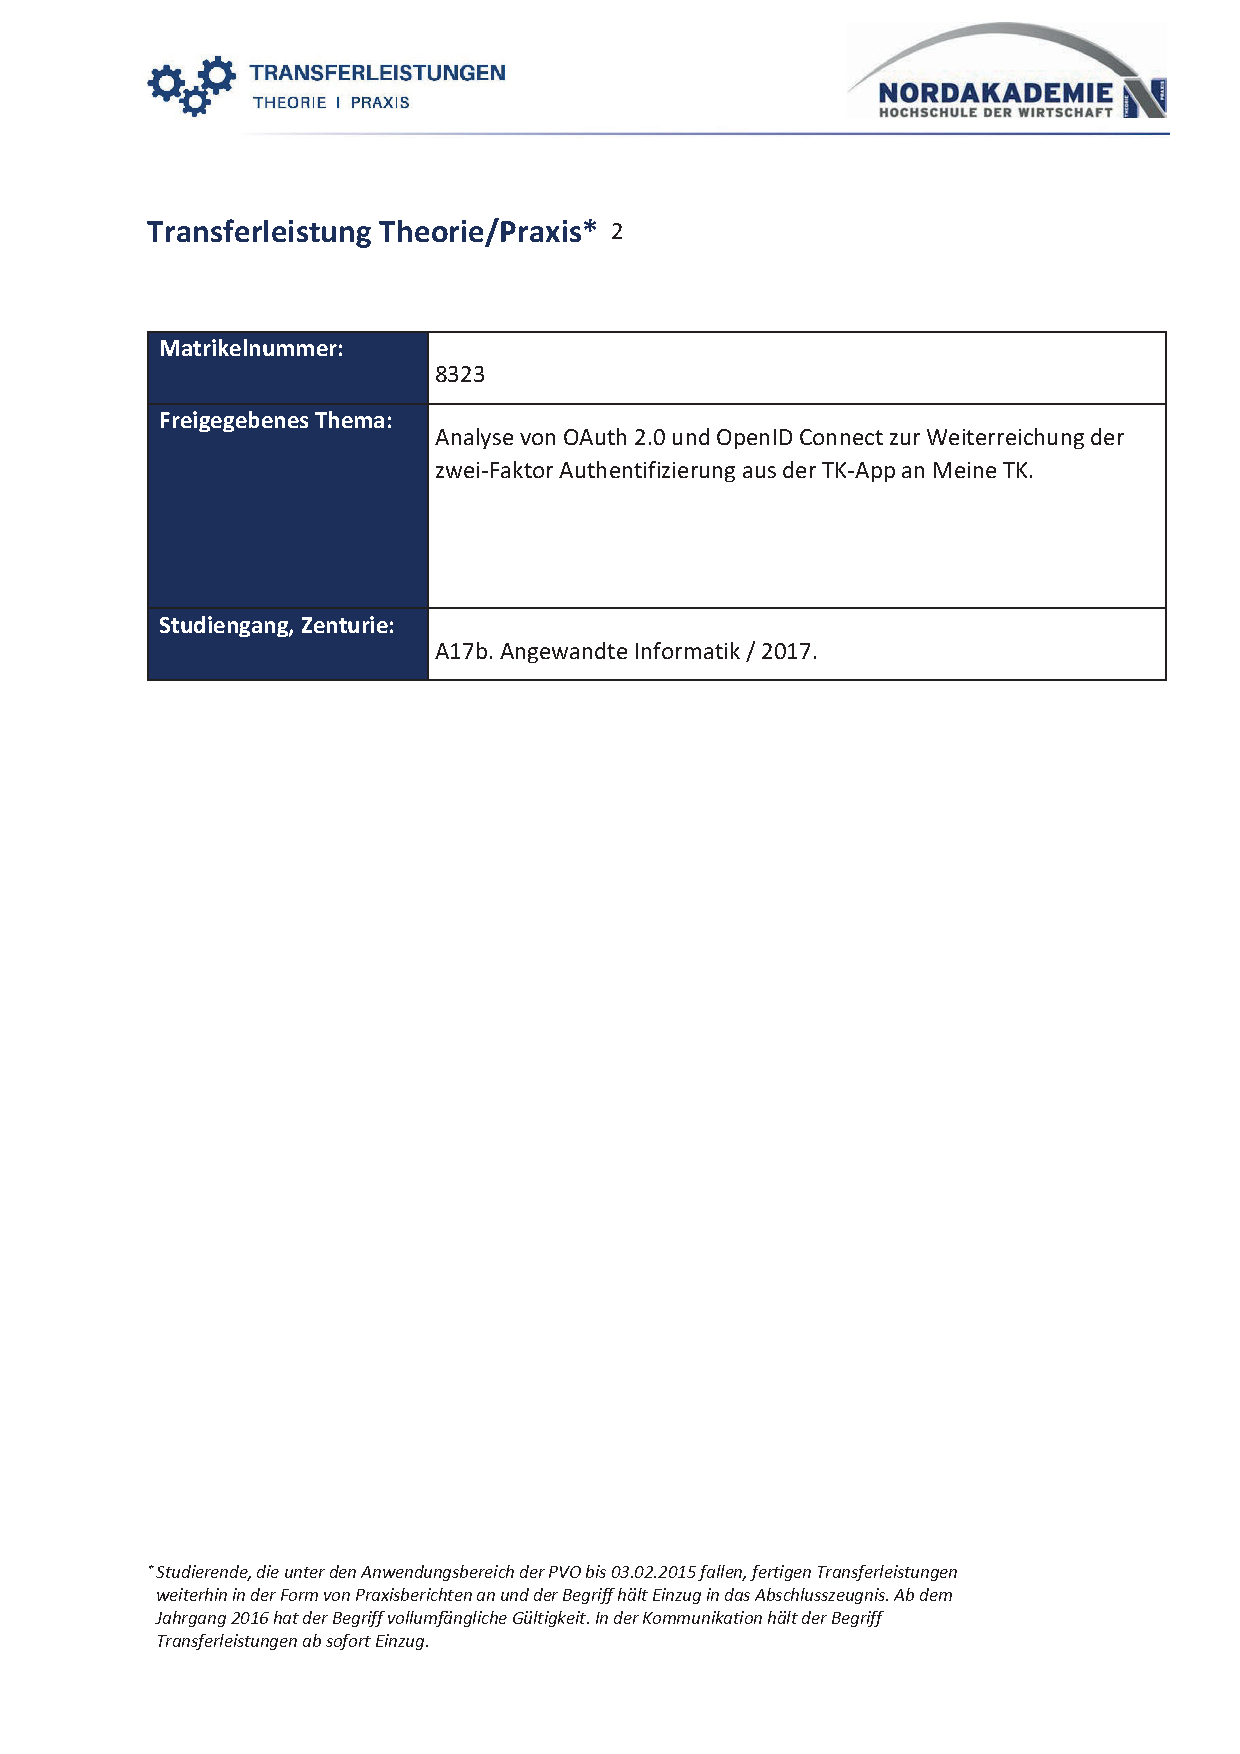
\includepdf[pages=1]{misc/deckblattTerminiert.pdf}

\begin{frontmatter}  %% Deckblatt, Abstract, diverse Verzeichnisse, Glossar.

  \listoftodos{}            % Aktuelle ToDo-Notes
  \newpage
  \tableofcontents        % Inhaltsverzeichnis
  \printglossaries{}      % Abkürzungsverzeichnis/Glossar
  \newpage
  \thispagestyle{empty}
  \addtocounter{page}{-4}
\listoftodos{}
\end{frontmatter}

\begin{mainmatter}
\chapter{Introduction}
\blindtext[3]
\todo{Generate a `class prototype' for stamp and no-stamp classes. (what is the
perfect stamp picture)}
\todo{Write a colour shifter for preprocessing, s.t. every colour is trained
and maybe even consider a color gradient shifter}

\chapter{Related Work}\label{chap:Related Work}
In the past, a variety of methods for stamp detection have been proposed.
A patent on page segmentation, a closely related topic, dates back as far as
1985 on Google Patents. A typical strategy found in most publications is to
first seperate a set of stamp-candidates from text and background, followed by
a verification of those candidates by applying thresholds on multiple
previously chosen features. To provide an overview of the topic, recent work on
stamp detection is split into two major- and several sub-categories.
\begin{description}
    \item [Restricted approaches]
        \begin{enumerate*}[label={\alph*)},font={\color{red!50!black}\bfseries}]
            \item [Color restricted]
                    In~\cite{Micenkova.18.09.201121.09.2011},
                    ~\citeauthor{Micenkova.18.09.201121.09.2011} present an
                    approach based on color clustering and geometric features.
                    To extract a set of stamp-candidates from a given image,
                    they assume stamps to be chromatic objects. In consequence,
                    all achromatic parts are dropped off the image. To seperate
                    the remaining candidates for individual analysis, the
                    XY-Cut algorithm proposed in~\cite{Krishnamoorthy.1993} is
                    applied. For classification an ensemble of geometric-
                    (pixel density, skew, etc.) and color-related features
                    (standard deviation of hue) is compared to empirically set
                    thresholds. By treating stamps as chromatic objects, they
                    are unable to detect black stamps and face problems when
                    colored fonts are used. In~\cite{Micenkova.2015},
                    \citeauthor*{Micenkova.2015} improved upon their method by
                    applying additional geometric features. Although
                    applicability of the updated approach on black stamps is
                    assumed, this hypothesis is not verified.\\A predecessor of
                    the approach in~\cite{Micenkova.18.09.201121.09.2011}
                    is~\cite{Forczmanski.2010} which employs less
                    verificationfeatures and is only applicable to blue or red
                    stamps.\\
                \item [Geometrically restricted]
                    An early geometric analysis technique was formulated by
                    ~\citeauthor*{Zhu.2006} in~\cite{Zhu.2006}, utilizing a
                    novel ellipse detection algorithm inspired by houghes
                    transform. However, this method is solely suitable for
                    elliptical stamps.
        \end{enumerate*}
    \item [Generic approaches]
    \begin{enumerate*}[label={\alph*)},font={\color{red!50!black}\bfseries}]
        \item [Geometric features]
        A more versatile method than in~\cite{Zhu.2006} was proposed in
        \cite{Ahmed.25.08.201328.08.2013, Ahmed.2016}.
        \citeauthor*{Ahmed.25.08.201328.08.2013} make use of advances in
        feature detectors and feature descriptors. In a first step, the
        image is binarized and connected components are extracted. For each
        connected component, feature key points and feature descriptors are
        computed via the FAST and ORB algorithms. In addition, bounding box
        height and width of each connected component are extracted.
        Verification is performed by comparing the extracted features of each
        connected component to a (remarkably) small training set. On the
        contrary,~\citeauthor*{Ahmed.25.08.201328.08.2013} notice low precision-
        and recall-rates, caused by their inability to recognize severely
        overlapping stamps.\\
        In~\cite{Nandedkar.16.12.201519.12.2015},
        \citeauthor*{Nandedkar.16.12.201519.12.2015} extend an approach they
        suggested in~\cite{Nandedkar.23.08.201526.08.2015}. They analyse spatial
        frequency components in document images, finding text to be the major
        contributor. In order to segment a given image, they first conceal
        text-components by removing objects with high spatial frequencies and
        further apply a Gaussian filter. To prevent textual stamps from being
        removed, a chromaticity threshold is applied on the removal of spatial
        frequency components. To identifiy stamp-candidates, mean-shift
        segmentation is applied. Small regions are filtered with an empirically
        set threshold, the largest region is considered to be the background.
        For verification of stamp-candidates, AlexNet is used, producing three
        classes (logo, stamp and noise) in the final dense layer. Even though
        untreated in the paper, the presented approach of filtering spatial
        frequency components faces limitations regarding black textual stamps
        which might turn out to be removed by the spatial frequency filter.\\
        \item [Mixed features]
        \citeauthor*{Dey.16.12.201519.12.2015} propose an outliers-based
        method in~\cite{Dey.16.12.201519.12.2015}. To segment a given image,
        it is seperated in foreground and background using binarization. To
        retain color information the obtained foreground-values are applied as
        a mask to the original image. Color information is reduced from
        three-dimensional \(RGB\) color space to a one-dimensional principal
        component using the Principal Component Algorithm (\(PCA\)).
        Stamp-candidates are obtained using a connected componets algorithm on
        the first principal component. To filter out false positives,
        thresholds on features such as stroke width, bounding box width and
        height are applied. For verification a set of features is extracted and
        validated using additional empirically set thresholds.\\

        A sliding window approach using the AdaBoost algorithm on cascaded
        decision trees has been proposed in~\cite{Forczmanski.2016}. In order
        to train AdaBoost, a labeled training set is constructed. For each
        training sample, haar-like features are extracted. AdaBoost then
        constructs a set of consecutive decision trees to optimize stamp
        classification of training samples. Each decision tree takes in a
        haar-like feature from a fixed position inside the sliding window.
        Based on the input feature value the tree decides whether to accept or
        reject a given window as stamp-candidate. A set of consecutive decision
        trees with such property (accept or completely reject) is called a
        cascade. In order for a sliding window to become a valid
        stamp-candidate it has to survive this cascade of decision trees. The
        set of generated candidates is then verified using a broader set of
        features. Several algorithms are compared for verification including
        1NN, decision trees, and SVMs.\\

        In~\cite{Younas.09.11.201715.11.2017},
        \citeauthor*{Younas.09.11.201715.11.2017} propose an approach using a
        Fully Convolutional Network (FCN), built upon the VGG-16 network
        architecture. In this approach, the final dense layers of VGG-16 are
        replaced a deconvolution layer. By doing this, a prediction map is
        received as output instead of classification scores. To reduce training
        time, transfer learning from the VOC2011 dataset is applied. However,
        no preprocessing is mentioned. Using 90\% of their dataset for training
        and 10\% for verification they report state-of-the-art results,
        although noticing difficulties with tabular stamps.
    \end{enumerate*}
\end{description}

Despite numerous research carried out on stamp segmentation, most of the 
approaches examined in this chapter either face limitations with overlapping 
objects~\cite{Nandedkar.23.08.201526.08.2015, Nandedkar.16.12.201519.12.2015, 
Forczmanski.2016, Ahmed.25.08.201328.08.2013, Dey.16.12.201519.12.2015, 
Forczmanski.2015, Forczmanski.2016} or logo misclassification~\cite
{Ahmed.25.08.201328.08.2013, Dey.16.12.201519.12.2015, 
Micenkova.18.09.201121.09.2011}, some approaches fall short\todo{falling short does not exactly fit here}
on runtime, operating for more than 13 Seconds per evaluation~\cite{Ahmed.2016, 
Nandedkar.23.08.201526.08.2015}.\\
Besides, classification of stamps is observed to be a common task in 
literature. Classes are usually either binary (Stamp and non-Stamp), 
object-related (Stamp, Logo, Text, Tables)~\cite{Forczmanski.2016,
Nandedkar.23.08.201526.08.2015, Nandedkar.16.12.201519.12.2015, 
Dey.16.12.201519.12.2015}, or shape-dependent (Circle, Ellipse, Square, etc.)
~\cite{Forczmanski.2015}. However, classification of similar stamps, i.e. 
stamps belonging to the same shape-class but differing in text and décor, as is 
often the case when dealing with different actors in business contexts, was not 
found.

\todo{Keine absoluten Aussagen.}
\todo{Deckblatt anpassen}
\todo{Arab. Nummerierung im Appendix, Backmatter?}
\todo{Datum auf dem Titelblatt ist denglisch}
\todo{Double check spatial frequency paper [8, 9]}
\todo{Glossar füllen, PCA etc.}
\todo{include kaggle approach}
\todo{extract best practices from dissertation}
\todo{Cite FAST and ORB, Gaussian, mean shift, PCA, K-NN, decision tree, SVM, 
VGG16, FCN, deconvolution, VOC2011?}
\todo{PCA is in math environment...}
\section{Methodology}\label{chap:Methodology}
To address the challenges identified in~\cref{chap:Related Work}, namely
evaluation-speed and categorization of near-classes, recent advances in machine
learning are considered. Contrary to most approaches in the field which perform
segmentation, this work focuses on detecting \glspl{bbox}. In this section,
details on the applied method is provided. Methods for object detection can coarsely
be divided into two groups: one-staged and two-staged approaches. To reduce complexity,
only a single one-stage approach will be considered in this paper. For details on
two stage detectors confer e.g.\ \cite{Ren.2015}.

\bigskip
{\large{\textbf{Single Shot MultiBox Detector}}}\\
Two common one-stage architectures are
\gls{yolo}~\cite{Redmon.2015, Redmon.2016b, Redmon.2018} and
\gls{ssd}~\cite{Liu.2016}. While \gls{ssd} can be extended to any base network
(e.g. VGG16~\cite{Simonyan.2015}), \gls{yolo} is limited to only Darknet~\cite{Redmon.2016}.
Therefore, \gls{ssd} was chosen over \gls{yolo} for this paper, retaining the
ability to quickly exchange base networks.

Central concepts of \gls{ssd} are described in the following.

\subsection{Default Boxes}\label{subsect:default-boxes}
The most fundamental part of understanding \gls{ssd} is understanding its specific
concept of \glspl{bbox}, default boxes and anchors. In order to reduce the very high
complexity, this subsection is written in a slightly more colloquial manner.

Slightly anticipating and simplifying \cref{subsect:SSD Architecture}, a
\emph{prediction} from \gls{ssd} is the output from a set of \glspl{convolutional layer}
that is chosen from within the network. Output of a single such \gls{layer} is,
first and foremost, just a \gls{feature map} --- while the goal is to find the
coordinates of a \gls{bbox} (and class predictions). 

Consider such a \gls{feature map} with dimensions \(m \times n\). Every pixel
from that \gls{feature map} contains highly condensed information about a specific
region from the original image\footnote{This concept is called the
\emph{receptive field} of \glspl{cnn}, \cite[cf.][331\psq]{Goodfellow.2016}}.
The \gls{feature map} is then processed further, s.t.\ for every such
pixel (and therefore the related region within the original image) receive the
coordinates of a single \gls{bbox} are received (simplified, for details see \cref{subsect:SSD Architecture}).

To the reader, this might be confusing. Receiving \(m\times n\)
single \gls{bbox} predictions for every pixel within the \gls{feature map} for
every chosen layer makes the number of predicted \glspl{bbox} \(\gg\) than the
expected number of \gls{gt} \glspl{bbox}. And it raises a pressing question:\linebreak
\textbf{How is training data constructed for such an unusual architecture?}

This question is answered (partly) by the introduction of \textbf{anchors}.

\paragraph{Anchors}\label{par:anchors}
Every pixel from a \gls{feature map} is related to a region within the original
input image (\emph{receptive field}~\cite[cf.][331\psq]{Goodfellow.2016}).
Furthermore, \glspl{convolutional layer} preserve the spatial structure of a
convolved image~\cite[cf.][335\psqq]{Goodfellow.2016}.

Therefore, every \emph{pixel} from within the feature map can be related
(very easily) to a region within the original image. The center of such region
is called the \textbf{anchor}. The x and y coordinates for every pixel \(p_{ij}\)
can then be calculated using \cref{eq:anch-x,eq:anch-y}. A practical example for an
image \(I\) of height and width \(I_w\times I_h=300\times 300\) and a
\gls{feature map} \(M\) of height and width \(M_w\times M_h=19\times 19\)
is shown in \cref{fig:vgg16-anchors}.

\begin{align}
    x_i&=0.5*\frac{w_I}{w_M} + \sum_{0}^{i-1} \frac{w_I}{w_M}\label{eq:anch-x}\\
    y_j&=0.5*\frac{h_I}{h_M} + \sum_{0}^{j-1} \frac{h_I}{h_M}\label{eq:anch-y}
\end{align}
where:
\begin{conditions}
    x_i & := & x-coordinates of the anchor for pixel \(p_{ij}\)\\
    y_j & := & y-coordinates of the anchor for pixel \(p_{ij}\)\\
    w_I & := & width of input image \(I\)\\
    w_M & := & width of feature map \(M\)\\
    h_I & := & height of input image \(I\)\\
    h_M & := & height of feature map \(M\)
\end{conditions}
\begin{figure}[t!]
    \centering
    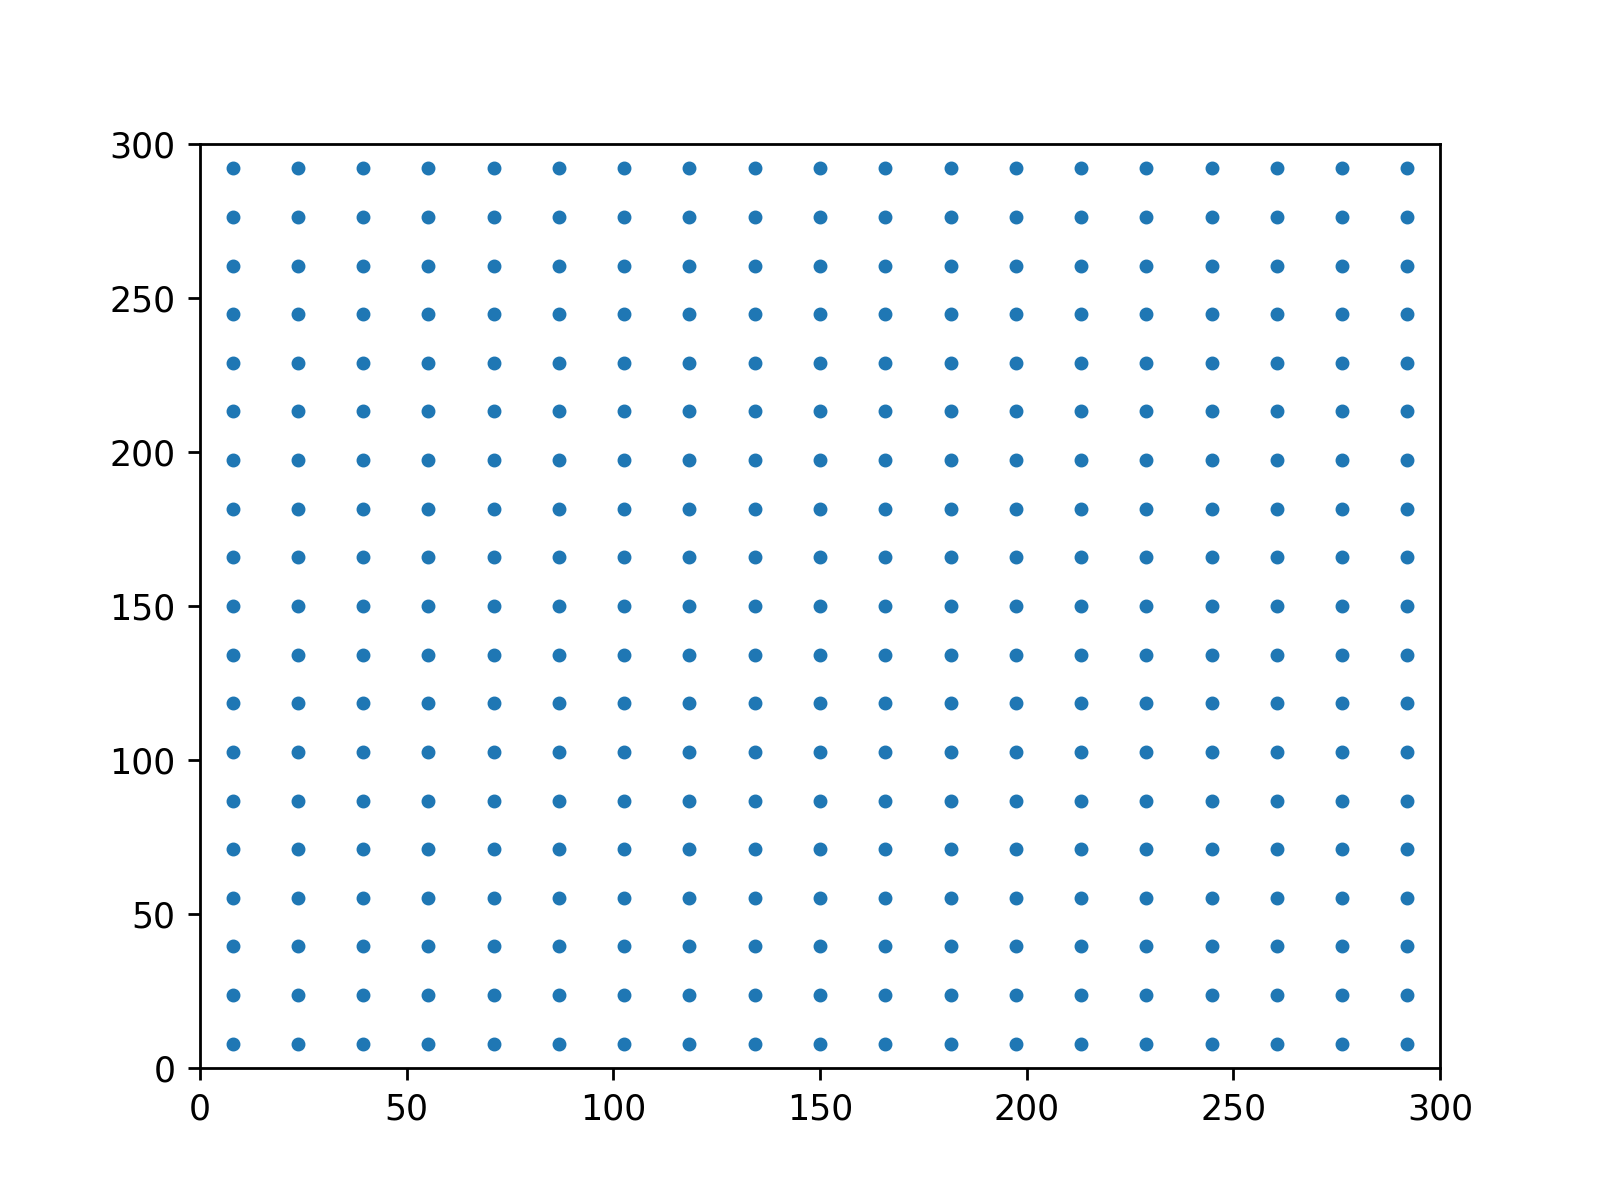
\includegraphics[width=0.5\textwidth]{vgg16-19x19}
    \caption{Generated anchors (blue) for an image of dimensions \(300\times 300\)
    and \gls{feature map} of \(19\times 19\).}\label{fig:vgg16-anchors}
\end{figure}
Now, training data could be constructed by assigning every \gls{gt} \gls{bbox} to
its closest anchor (from every chosen layer). An example of this is given in
\cref{eq:train-anchor}. 
\begin{equation}\label{eq:train-anchor}
    \begin{matrix}
        \ldots\\
        \begin{bmatrix}
            \ldots & \ldots & \ldots & \ldots & \ldots\\
            0 & 0 & 0 & 0 & 0\\
            271 & 828 & 182 & 845 & 1\\
            0 & 0 & 0 & 0 & 0\\
            \ldots & \ldots & \ldots & \ldots & \ldots
        \end{bmatrix}\\
        \ldots\\
        \begin{bmatrix}
            \ldots & \ldots & \ldots & \ldots & \ldots\\
            0 & 0 & 0 & 0 & 0\\
            3141 & 592 & 653 & 59 & 1\\
            0 & 0 & 0 & 0 & 0\\
            \ldots & \ldots & \ldots & \ldots & \ldots
        \end{bmatrix}\\
        \ldots
    \end{matrix}
\end{equation}
where the first four rows are x- and y-coordinate, height and width of the respective
\gls{bbox} and the last row is the class (0: \textit{no-object}, 1: \textit{object}).

This approach is flawed in two ways:
\begin{enumerate}
    \item Assigning \gls{gt} \glspl{bbox} to the closest anchor is entirely agnostic
    of the expected size of the receptive field for the different layers. A layer
    with smaller receptive field per pixel would probably not be able to perceive
    larger objects, while a layer with a larger receptive field might overlook
    smaller objects.\label{itm:anchor-flaw1}
    \item The model has no \textit{a priori} knowledge of \emph{position}, of
    \emph{x-} and \emph{y-coordinates}, of \emph{width} and \emph{height}.
    This is especially critical for images with different resolutions.\label{itm:anchor-flaw2}
\end{enumerate}
A possible solution to these flaws are \textbf{default boxes}.

\paragraph{Default Boxes}\label{par:default-boxes}
Default boxes are used to assign spatial representation to anchors. With such a
representation, every \gls{gt} \gls{bbox} can be matched to the set of regions
(related to the receptive fields) that have a large overlap\footnote{The overlap
could then be computed via \gls{iou} for example --- as is done in \cref{eq:bbox-matcher}.}.

As a starting point, so far a set of chosen layers \(L = \left\{l_0, l_1, \ldots, l_{n-1}\right\}\)
and a set of anchors for every such layer \(\mathbf{A} = \left\{A_0, A_1, \ldots, A_{n-1}\right\}\)
were constructed.

Now, although the exact receptive fields of the chosen layers are uncertain, 
we \emph{do} know that their sizes \(\abs*{recept\left(l\right)}\), are strictly
increasing with subsequent layers, i.e.\ \(\abs*{recept\left(l_0\right)} < \ldots < \abs*{recept\left(l_{n-1}\right)}\).

Fortunately, \textcite{Liu.2016} claim that the exact size of the receptive field is of
subordinate importance. Instead of calculating the exact receptive field, they
propose to assign a fixed size to every chosen \gls{layer} per \cref{eq:default-box-size}:
\begin{equation}\label{eq:default-box-size}
    s_k=s_{_\text{min}} + k * \frac{s_{_\text{max}}-s_{_\text{min}}}{n-1}
\end{equation}
Where
\begin{conditions}
    n               &:= & \(\abs*{L}\)\\
    k               &\in & [0, n-1]\\
    s_{_\text{min}} &=& 0.2\\
    s_{_\text{max}} &=& 0.9
\end{conditions}
A default box \(d_{i,j}\) for a pixel \(p_{i,j}\) within a given layer \(l_k\)
can then be computed as given in \cref{eq:dbox}.
\begin{align}
    \begin{split}\label{eq:dbox}
        d_{i,j}^h  &= s_k * h_I\\
        d_{i, j}^w &= s_k * w_I\\
        d_{i,j}^x  &= x_i \text{ (see \cref{eq:anch-x})}\\
        d_{i,j}^y  &= y_j \text{ (see \cref{eq:anch-y})}
    \end{split}
\end{align}
It is now possible to match every \gls{gt} \gls{bbox} to a set of default boxes
(see \cref{eq:bbox-matcher}).
\begin{equation}\label{eq:bbox-matcher}
    match(\text{bbox}, \text{dbox}) =
    \begin{cases}
        1 & \text{if } \text{IoU}\left(\text{bbox, dbox}\right) > 0.5\\
        0 & \text{otherwise}
    \end{cases}
\end{equation}
where:
\begin{conditions}
    \text{bbox} & := & coordinates of the bounding box\\
    \text{dbox} & := & coordinates of the default box
\end{conditions}
Thereby, \hyperref[itm:anchor-flaw1]{\(\left.\text{flaw 1}.\right)\)} from anchor
construction can be considered as solved.

\hyperref[itm:anchor-flaw2]{\(\left.\text{Flaw 2}.\right)\)} can now be tackled
multiple ways. The most obvious would be to convert \gls{gt} \glspl{bbox} and
default boxes into the \textit{percental} space (i.e. \(\left[0, 1\right]\)).
Yet, this again would require the model to learn different semantics per pixel
within a \gls{feature map}. For example, the upper left pixel/region would produce predictions
within \(\left[0,0.2\right]\times \left[0,0.2\right]\), while the lower right
region would produce predictions within \(\left[0.8,1.0\right]\times \left[0.8,1.0\right]\).
This is problematic, because \glspl{convolutional layer} share weights\footnotemark{}
between inputs (i.e. such pixels/regions)~\cite[cf.][564\psqq]{Murphy.2012}.
\footnotetext{In fact, sharing weights between inputs is the key distinguishing
feature between \glspl{convolutional layer} and \glspl{dense layer}.}
Requiring different semantics \emph{between} these pixels introduces additional
complexity to the \glspl{convolutional layer}.

To alleviate this complexity, rather than coordinates, the offset \emph{between}
the coordinates (of \gls{gt} \glspl{bbox} and the related default boxes) are predicted.
This aligns the task between all pixels of a \gls{feature map}.

\Textcite{Liu.2016} introduce a last quirk inspired by the concept of priors
from bayesian statistics~\cite[cf.][165\psqq]{Murphy.2012}. To improve convergence
they choose multiple aspect ratios (i.e.\ 1:1, 1:2, 1:3, 2:1, 3:1) for their
default boxes. Reducing extent of this paper, the reader is referred to \cite{Liu.2016}.

Finally, the sets of default boxes per \gls{layer} are concatenated and further
encoded as described in \cref{append:Concepts of Bounding Box Encoding}, such
that default box

\subsection{Encoding Ground Truth} For training, ground truth \glspl{bbox}
are encoded with respect to the concatenated default boxes as calculated in
\cref{par:default-boxes}. 


\gls{ssd} is supposed to infer offsets to default
boxes (cf. \cref{subsect:SSD Architecture}). To simplify inference only default
boxes with an \gls{iou} greater than 0.5 are chosen (cf. \cref{sect:Intersect Over Union}). For a \gls{bbox}
\(\text{bbox}=\{\text{bbox}_{x_\text{min}}, \text{bbox}_{x_\text{max}}, \text{bbox}_{y_\text{min}}, \text{bbox}_{y_\text{max}}\}\), default box
\(\text{dbox}=\{\text{dbox}_{x_\text{min}}, \text{dbox}_{x_\text{max}}, \text{dbox}_{y_\text{min}}, \text{dbox}_{y_\text{max}}\}\) we compute the
encoded box \(\text{ebox}\) with \cref{eq:encoded box}
\begin{equation}
    \text{ebox}=\{(\text{bbox}_{x_\text{min}}-\text{dbox}_{x_\text{min}}), (\text{bbox}_{x_\text{min}}-\text{dbox}_{x_\text{max}}), (\text{bbox}_{y_\text{min}}-\text{dbox}_{y_\text{max}})\}\label{eq:encoded box}
\end{equation}
We receive a matrix of dimensions \(\sum_{m\in M}{A_m}\times \sum_{m\in M}{k_m*4}\),
where \(M\) is the set fo all \glspl{feature map}, \(A_m\) is the set of all anchors per
\gls{feature map} and \(k_m\) is the amount of aspect ratios per \gls{feature map}. Finally
we concatenate the class label to every encoded \gls{bbox}, such that the matrix
dimensions now are \(\sum_{m\in M}{A_m}\times \sum_{m\in M}{k_m*4+c}\), where c
is the amount of classes. Every row is now in the form of
\begin{equation}
    \left\{x_{_\text{min}}, x_{_\text{max}}, y_{_\text{min}}, y_{_\text{max}}, \text{one\_hot\_classes} \right\}
\end{equation}


\subsection{SSD Architecture}\label{subsect:SSD Architecture}
As mentioned in the introduction to this section, \gls{ssd} is independent of any
specific base network. Exemplary, \cref{fig:ssd-vgg} shows the architecure of
SSD for VGG16~\cite{Simonyan.2015}. Fully connected \glspl{layer} of VGG16 are
dropped and replaced with additional \glspl{convolutional layer}. We denote: 
\(\text{Network}:=\text{Base Network}\rightarrow \text{Additional Layers}\).

Then, a set of \glspl{convolutional layer} \(L\) (blue and yellow in \cref{fig:ssd-vgg})
is chosen from the network (i.e.\ \(L\subseteq \text{Network}\))\footnote{\label{foot:receptive}The motivation
behind choosing multiple layers \(L\) from the network is as follows: the \glspl{feature map}
produced by the \glspl{convolutional layer} get smaller with every additional layer.
Colloquially speaking, the relationship between such a small \gls{feature map} and
the input image is, that one pixel within the small \gls{feature map} is related
to multiple pixels within the original input image. Therefore, when looking at the
\glspl{feature map} from subsequent \glspl{convolutional layer}, one is looking
at information that is extracted from the image at different scales.

Making this logic concrete, in a larger \gls{feature map}, one pixel might contain
condensed information about objects like wheels or headlights, whereas in a smaller
\gls{feature map} one pixel might contain  condensed information about the entire
car. This concept is called the \textit{receptive field}~\cite[cf.][331\psq]{Goodfellow.2016}.}.

To produce class- and \gls{bbox} predictions, every chosen \glspl{layer} \(l\in L\)
is directed into a final additional \gls{convolutional layer} (i.e.\ one additional
\gls{convolutional layer} per \gls{layer} in \(L\), depicted green in \cref{fig:ssd-vgg}).

Das hier setzt halt alles Wissen voraus, das noch gar nicht aufgebaut wurde!

The number of filters for these subsequent \glspl{layer} is chosen as \((4+c)*k\)
with \(c\) classes\footnote{Actually, \(c+1\) classes. This additional class is
the \textit{no-class}-prediction, because obviously most areas within the image
contain no classifiable object.} and \(k\) default boxes per \gls{anchor}.
\begin{figure}[ht]
    \centering
    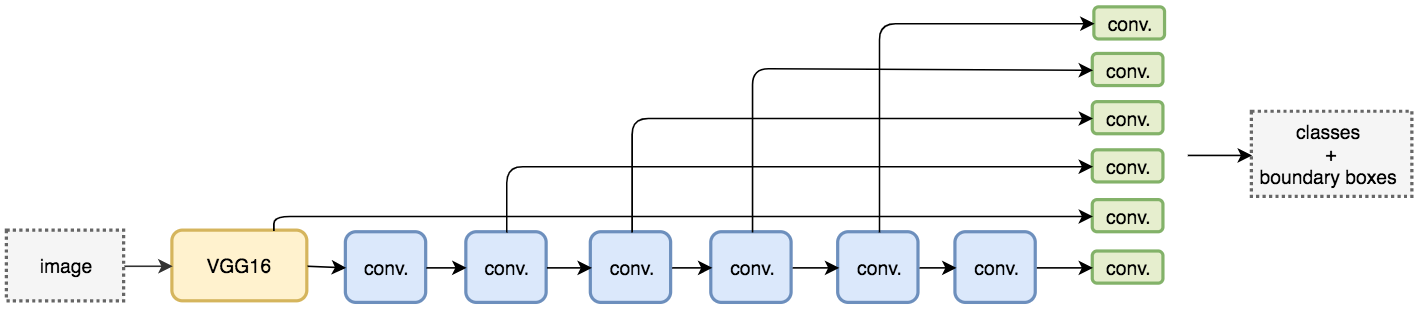
\includegraphics[width=1\textwidth]{vgg16-ssd}
    \caption[Example of the SSD architecture using VGG16 as its base network]{Example
    of the SSD architecture using VGG16 as its base network~\cite[cf.][]{Liu.2016}.
    \\\\
    Blue colored boxes represent the additional \glspl{convolutional layer} that are added to the base network.
    \\\\
    Green boxes represent the final additional \glspl{convolutional layer} that produce
    the classes- and \gls{bbox} predictions.}
    \label{fig:ssd-vgg}
\end{figure}

\subsection{Training}
\ldots

\subsubsection{Loss Function}
The loss is a composite of two separate loss functions:

\begin{align}
    L_{\text{conf}(x, c)}\\
    L_{\text{loc}(x, l, g)}\\
    L(x,c,l,g) = \frac{1}{N}*\left(L_{\text{conf}(x, c)} + \alpha * L_{\text{loc}(x, l, g)}\right)
\end{align}

\begin{equation}
    \begin{cases}
        L(x,c,l,g) = \frac{1}{N}*\left(L_{\text{conf}(x, c)} + \alpha * L_{\text{loc}(x, l, g)}\right),& \text{if } N \geq 1\\
        0, & \text{otherwise}
    \end{cases}
\end{equation}

\begin{equation}
    L_{\text{loc}(x, l, g)} = \sum_{i \in Pos }^{N}
\end{equation}
where:
\begin{conditions}
    N & := & number of matched boxes\\
    x & := & pixel under consideration\\
    c & := & class scores\\
    l & := & Predicted Boxes\\
    g & := & Ground Truth Boxes\\
    \alpha & := & weighting parameter, increase to put importance on the localization loss.
\end{conditions}

\section{Experimental Results}
This chapter gives an overview of the applied dataset (\cref{sect:staver})
and experimental setup (\cref{sect:exp-setup}). Finally, the results are discussed
in \cref{sect:results-and-discussion}. For the interested reader, an introduction
to the applied metric (\gls{map}) is provided in \cref{sect:metrics}.

\subsection{StaVer}\label{sect:staver}
\Gls{ssd}, as presented in \cref{sect:methodology} will be evaluated on the publicly
available dataset \gls{staver}\footnotemark~\cite{Micenkova.2015}.
\footnotetext{\url{https://madm.dfki.de/downloads-ds-staver}}

From direct examination, the dataset contains 427 images in total. However,
27 images are not annotated and can therefore not be used for train/test splits.
Out of the remaining 400 images, 320 images contain colored and the remaining
80 images contain black stamps.  To reduce computational complexity, a resolution
of 200 dpi is chosen, although 300 and 600 dpi are also available. The dataset
comprises several stamp-categories. Most distinctly, graphical and textual stamps
are included. As an addition to the original dataset, the author has produced
class annotation (``Text'', ``Image'').

For every image, two different \gls{gt} types are available. The former contains
a segmentation map\footnotetext{Meaning that every pixel belonging to a stamp is
marked.}, the latter \gls{gt} \glspl{bbox}. Unfortunately, both given \gls{gt}
types are provided only in form of images \cref{fig:text-stamp-gt,fig:img-stamp-gt}.

Coordinates (as required for \cref{eq:offset-calc}) are extracted from the \gls{gt}
\gls{bbox} images programmatically. OpenCV~\cite{Bradski.2000} is used to find
connected components and convert them into rectangles. Finally, coordinates are
determined using \texttt{cv2.boxPoints(\ldots)}.

\begin{figure}[th!]
    \begin{subfigure}[t]{.225\linewidth}
        \centering
        \includegraphics[width=.9\textwidth]{stampDS-00251.png}
        \subcaption{Textual stamp example from \gls{staver} (stampDS-00251)}\label{fig:text-stamp}
    \end{subfigure}\hfill
    \begin{subfigure}[t]{.225\linewidth}
        \centering
        
\includegraphics[width=.9\textwidth]{stampDS-00251-gt.png}
        \subcaption{Image containing the \gls{gt}\gls{bbox} for the textual stamp (stampDS-00251)}\label{fig:text-stamp-gt}
    \end{subfigure}\hfill
    \begin{subfigure}[t]{.225\linewidth}
        \centering
        \includegraphics[width=.9\textwidth]{stampDS-00138.png}
        \subcaption{Two image-stamps from \gls{staver} (stampDS-00138)}\label{fig:img-stamp}
    \end{subfigure}\hfill
    \begin{subfigure}[t]{.225\linewidth}
        \centering
        
\includegraphics[width=.9\textwidth]{stampDS-00138-gt.png}
        \subcaption{Image containing the \gls{gt}\gls{bbox} for the two image-stamps (stampDS-00138)}\label{fig:img-stamp-gt}
    \end{subfigure}
    \caption[Example images from \gls{staver} and respective \gls{gt}]{Example
    images from \gls{staver} and respective \gls{gt} \glspl{bbox}. Unfortunately,
    \gls{bbox} \gls{gt} is sometimes corrupted, e.g.\ (\subref{fig:img-stamp-gt}).}
\end{figure}

\subsection{Experimental Setup}\label{sect:exp-setup}
For image preprocessing, a set of manipulations
\begin{multline*}
    \{\text{Brightness-jitter, Color-jitter, Saturation-jitter, Horizontal-flip, Vertical-flip, Random-crop,}\\\text{Black-and-White}\}
\end{multline*}
are applied randomly.

\Gls{ssd} is implemented by the author using Python 3.7 and TensorFlow 2.0~\cite{Abadi.2015}.
As base network, MobileNet~\cite[cf.][]{Howard.2017} is adopted without pre-training\footnotemark.
Hyperparameters are chosen as per the original paper, confer~\cite{Liu.2016}.
Training and inference are run using \texttt{NVIDIA DGX A100} infrastructure.

\footnotetext{Common datasets like e.g.\ ImageNet~\cite{Deng.2009} come from a substantially different
distribution. Note please that pre-training and thereby heterogenous transfer learning
\textit{might} be useful nonetheless~\cite{Day.2017}, but would require additional
ablation studies which is beyond the scope of this work.}

Out of the 400 available and annotated images, 65\% (240) are chosen for training
and 35\% (100) are chosen for testing. A validation set is not constructed, because
no hyperparameter optimization is conducted~\cite[cf.][120\psq]{Goodfellow.2016}.

\subsection{Results \& Discussion}\label{sect:results-and-discussion}
Results seem generally competitive with the original implementation by \textcite{Liu.2016}\footnotemark.
Besides that, the results from this work unfortunately cannot be compared to
related approaches in stamp detection which, as noted in \cref{sect:related-work},
were mostly concerned with image segmentation.

As demonstrated in \cref{fig:loss,fig:map-75}, the model converges after about
a 10.000 training steps, reaching its maximum \gls{map}@0.75\gls{iou} of 0.593
after 9.000 training steps.

\footnotetext{Comparing apples and oranges, the best implementation of \gls{ssd}
by \textcite{Liu.2016} reached a \gls{map}@.75\gls{iou} of 30.3[Table 6, \texttt{COCO test-dev2015}]\cite{Liu.2016}.}

\begin{figure}[htp!]
    \centering
    \begin{subfigure}{.49\linewidth}
        \begin{tikzpicture}
            \begin{axis}[cycle list name=tb, 
                        grid=both,
                        grid style={solid,gray!30!white},
                        axis lines=middle,
                        xlabel={step},
                        ylabel={L(l)},
                        x label style={at={(axis description cs:0.5,-0.1)},anchor=north},
                        y label style={at={(axis description cs:-0.1,.5)},rotate=90,anchor=south},]
            \addplot table [x=Step, y=Value, col sep=comma] {loss.csv};
            \end{axis}
        \end{tikzpicture}
        \subcaption{Model loss over time}\label{fig:loss}
    \end{subfigure}
    \hfill
    \begin{subfigure}{.49\linewidth}
        \begin{tikzpicture}
            \begin{axis}[cycle list name=tb, 
                        grid=both,
                        grid style={solid,gray!30!white},
                        axis lines=middle,
                        xlabel={step},
                        ylabel={mAP@75IoU},
                        ytick={0.3,0.4,0.5,0.595},
                        x label style={at={(axis description cs:0.5,-0.1)},anchor=north},
                        y label style={at={(axis description cs:-0.1,.5)},rotate=90,anchor=south},]
            \addplot table [x=Step, y=Value, col sep=comma] {map@75iou.csv};
            \end{axis}
        \end{tikzpicture}
        \subcaption{\gls{map}@.75\gls{iou} computed on the test set}\label{fig:map-75}
    \end{subfigure}
    \caption{Model loss and test metrics over time}
\end{figure}

From visual evaluation, the model is able to overcome most issues noted in
\cref{sect:related-work}. In most cases, black and white stamps could be
identified (see \cref{fig:black-and-white}) as well as stamps with significant
overlap (\cref{fig:diff-domain-overlap,fig:overlap-insample}).

As a downside it is noted that in few cases, \gls{ssd} was vulnerable to
\gls{fp} detections of logos, which look very similar to graphical stamps
(see \cref{fig:logo-as-stamp}). Also, sometimes multiple stamps are detected as
a single stamp (see \cref{fig:multi-as-one}).

Interestingly, also stamps from different distributions could be identified without
significant increase in \glspl{fp} (see \cref{fig-diff-domains}).

\section{Conclusion}
In this paper, \gls{ssd}~\cite{Liu.2016} has been thoroughly explained, implemented
by the author and applied on a publicly available dataset (\gls{staver}~\cite{Micenkova.2015}).
The achieved results were generally good and the method was able to overcome
several issues reported in previous work (see \cref{sect:related-work}).

\subsection{Future Research}
While the results were generally good, interesting ablation studies could include
the use of more powerful base networks (NASNetLarge~\cite{Zoph.2018},
InceptionResNetV2~\cite{Singh.2017}, \ldots). It would also be interesting to
observe how well \gls{ssd} performs on a dataset with exclusively black-and-white
images.

Finally, hyperparameters could be tuned using e.g.\ grid search~\cite[432-434]{Goodfellow.2016}
or Bayesian optimization~\cite{Agnihotri.2020}. Default box aspect ratios could
be picked by observing the histogram of all aspect ratios and pick the \mathvar{n}
most common aspect ratios.

Another interesting area of research would be the adaptation of heatmaps~\cite{Marban.2021}
to explain the predictions produced by the \gls{ssd} framework.
\todo{Mention Buda 2018, A systematic study of the class imbalance problemin convolutional neural networks}
\end{mainmatter}

\begin{appendices} %% Anhänge die nicht zwingend für die Arbeit notwendig sind
\chapter{Basic Concepts}\todo{Exchange for a better title}
\blindtext[1]

\section{Concepts of Bounding Box Encoding}
\blindtext[2]

\section{Preprocessing}
\blindtext[3]

\section{Concepts of Neural Network Architectures}
\blindtext[4]

\section{Loss Functions}
\blindtext[2]

\section{VGG16 and ResNet}
\blindtext[3]


%\chapter{General Todos}
\todo{Keine absoluten Aussagen.}
\todo{Deckblatt anpassen}
\todo{Arab. Nummerierung im Appendix, Backmatter?}
\todo{Double check spatial frequency paper [8, 9]}
\todo{Glossar füllen, PCA etc.}
\todo{extract best practices from dissertation}
\todo{Cite FAST and ORB, Gaussian, mean shift, PCA, K-NN, decision tree, SVM, 
VGG16, FCN, deconvolution, VOC2011?}
\todo{PCA is in math environment\dots}
\todo{Generate a `class prototype' for stamp and no-stamp classes. (what is the
perfect stamp picture)}
\todo{Write a colour shifter for preprocessing, s.t. every colour is trained
and maybe even consider a color gradient shifter}
\todo{Why combine localization and classification, why not split both? Is it speed only?}

\end{appendices}

\begin{backmatter} %% bibliography, tables of figures etc., index...)
% Consider colophon  
%% You’re recommended to use the eprint-aware biblio styles which
%% can be obtained from e.g. www.arxiv.org. The file mythesis.bib
%% is derived from the source using the SPIRES Bibtex service.
\printbibliography{}  %% Literaturverzeichnis
%% I prefer to put these tables here rather than making the
%% front matter seemingly interminable. No-one cares, anyway!
\listoftables           % Tabellenverzeichnis
\listoffigures          % Abbildungsverzeichnis
\end{backmatter}

\end{document}
